\section*{\Large{Введение}}
\addcontentsline{toc}{section}{Введение}

В современном мире каждая компания хочет минимизировать свои затраты, как по времени, так и в финансовом плане.
Это не обошло и сферу строительства.
В данной области существует ряд открытых задач, требующих решения,
в том числе это касается строительства различных площадных объектов.

Любому строительству предшествует этап проектирования.
Результатом этого этапа является генеральный план площадного объекта,
на основе которого можно оценить, как капитальные затраты, так и эксплуатационные.

\begin{wrapfigure}{r}[0pt]{0.5\textwidth}
    \begin{center}
        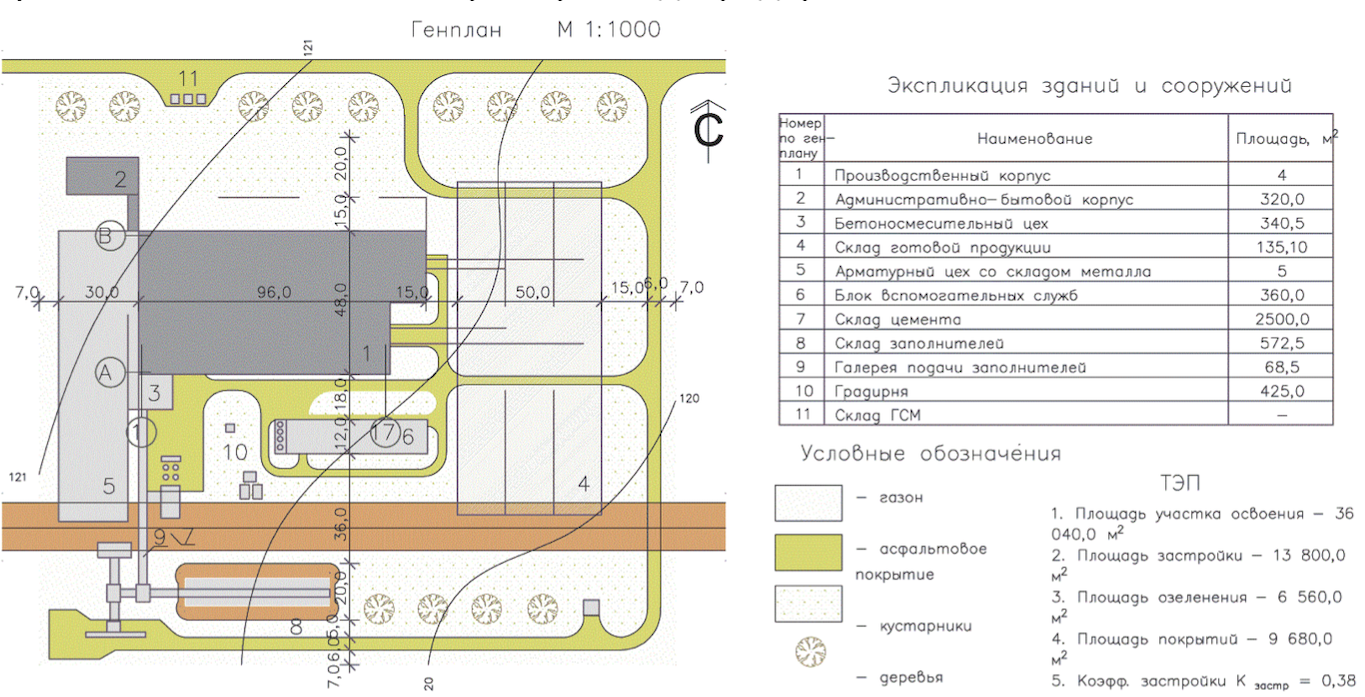
\includegraphics[width=\textwidth]{introduction/pictures/site_plan}
    \end{center}
    \caption{Генеральный план площадного объекта}
    \label{pic:problem__site-plan}
\end{wrapfigure}

За проектирование крупных объектов отвечают проектные институты.
При составлении проекта инженеры-проектировщики опираются на собственный опыт, а также на набор строительных норм
и правил эксплуатации.
В качестве основного рабочего инструмента используются CAD-системы.
В данных инструментах отсутствует, как механизм интерактивного вычисления стоимости получаемого решения,
так и возможность полностью автоматизировать процесс построения конструкции. Инженер строит решение вручную.


Создание системы подобного класса требует проведения массы научных исследований в сфере алгоритмов.
Но алгоритмы работают с математическими абстракциями.
А инженеры с конкретными объектами, такими как трубопроводы, линии электропередач и прочее.
Процесс обмена опыта между исследователями и инженерами это крайне непростое мероприятие,
требующее механизмов преобразования математических абстракций в объекты реального мира.

Получение качественной обратной связи позволяет достигать высоких результатов в исследованиях, а оперативность
позволяет это делать в короткие сроки.
